% 中文研究工作稿；正文事实与英文稿、生成表格及审计记录对齐。
% Compile: tectonic paper_zh.tex (requires a Chinese font; PDF embeds fonts).
\documentclass[11pt,a4paper]{article}
\usepackage[margin=24mm]{geometry}
\usepackage{fontspec,xeCJK}
\setmainfont{Times New Roman}
\setmonofont{Menlo}[Scale=MatchLowercase]
\IfFontExistsTF{Songti SC}
  {\setCJKmainfont{Songti SC}}
  {\setCJKmainfont{FandolSong-Regular}[BoldFont=FandolSong-Bold]}
\usepackage{amsmath,amssymb,mathtools}
\usepackage{booktabs,multirow,array,makecell}
\usepackage{graphicx}
\usepackage{natbib}
\usepackage{hyperref,cleveref}
\usepackage{enumitem}
\usepackage{tikz}
\usetikzlibrary{arrows.meta,positioning}
\setlist{noitemsep,topsep=3pt,leftmargin=*}
\hypersetup{colorlinks=true,linkcolor=blue,citecolor=blue,urlcolor=blue,
  pdfauthor={屈占祥 / Zhanxiang Qu},
  pdftitle={LLM团队需要多少通信？轻量消息门控的实证研究}}
\crefname{table}{表}{表}
\Crefname{table}{表}{表}
\crefname{figure}{图}{图}
\Crefname{figure}{图}{图}
\crefname{section}{节}{节}
\Crefname{section}{节}{节}
\crefname{appendix}{附录}{附录}
\Crefname{appendix}{附录}{附录}
\renewcommand{\abstractname}{摘要}
\renewcommand{\refname}{参考文献}
\renewcommand{\tablename}{表}
\renewcommand{\figurename}{图}
\sloppy
\emergencystretch=2em
\setlength{\hfuzz}{0pt}
\setlength{\parskip}{3pt}
\title{LLM团队需要多少通信？\\轻量消息门控的实证研究}
\author{屈占祥（Zhanxiang Qu）\\独立研究者\\
  \href{mailto:zhanxiangqu@126.com}{\texttt{zhanxiangqu@126.com}}\\
  \href{https://orcid.org/0009-0000-0137-9751}{ORCID: 0009-0000-0137-9751}}
\date{}

\begin{document}
\maketitle
\begin{abstract}
多智能体大语言模型系统是否需要广播每条候选消息？更复杂的门控是否优于简单冗余过滤？本文以信息瓶颈思想启发的VIB-Sparse为测试策略，在HumanEval（164题）、GSM8K（1319题）和MATH（5000题）上分析通信与任务表现。相对完整通信，HumanEval和GSM8K的广播消息减少21.14\%和30.49\%，精度差为$-1.83$和$-0.08$个百分点；MATH在保守完整答案匹配下差值为$-0.92$个百分点，广播减少25.59\%。GSM8K和MATH记录的总Token减少仅为4.96\%和4.42\%；HumanEval刷新代码沿用旧费用字段，不能声称完整成本节省。历史MBPP结果因参考测试参与早停而作为oracle-only证据隔离。三个早期HumanEval正收益批次通过实际重评，但不足以证明稳定优越性。另一个200题GSM8K子集上，余弦阈值门控与VIB的精度点估计均为97.00\%，配对差值区间为$[-2.50,+2.50]$个百分点。结果支持审慎的精度--成本评估和协议修复，不支持VIB特有优越性、正式等效性或可部署的讨论调度器结论。
\end{abstract}
\noindent\textbf{关键词：}多智能体大语言模型；稀疏通信；信息瓶颈；成本评估；实验可复现性。

\paragraph{版本说明。}
本文为可独立阅读的中文研究工作稿，内容与英文稿的事实和评分口径对应，而非逐句翻译。当前不是完成独立确认实验的正式投稿版本。生成表格是数值事实源；作者已确认无资助、无利益冲突，公开数据声明尚须投稿前复核。

\section{引言}
多智能体系统将代码生成、测试建议和验证等工作分配给不同角色，常通过共享历史广播所有候选消息。ChatDev、MetaGPT、AgentCoder和SWE-agent等工作展示了角色分工的不同形式\citep{qian2023chatdev,hong2023metagpt,du2023agentcoder,yang2024sweagent}。但是，更多讨论既可能补充推理，也可能传播错误建议；消息进入上下文并不代表它对最终正确性有贡献。

本文区分两个问题。第一，\textbf{上下文质量}：删除重复或错误内容是否能改善答案，需要控制候选内容的因果实验，而不是仅根据相似度分数推断。第二，\textbf{广播与实际费用}：如果候选已经生成，随后丢弃不能撤销其生成费用；节省的是可能减少的后续输入上下文，而非已发生的请求。

VIB-Sparse是信息瓶颈思想启发的确定性嵌入启发式。其名称不表示已经拟合、优化或证明变分互信息界。本文的贡献为：
\begin{enumerate}
\item 报告三个非oracle主基准的精度--广播权衡，并隔离参考辅助早停的MBPP历史结果。
\item 在相同任务和接近消息预算下比较Random、余弦阈值和VIB，不将消息数匹配误称为总费用匹配。
\item 审计评分、参数透传、合成刷新和成本关联，保留真实历史正收益，同时区分探索证据与稳定方法优势。
\end{enumerate}

\section{方法}
\subsection{任务与工作流}
HumanEval采用可执行代码测试\citep{chen2021evaluating}；历史MBPP-Sanitized采用顶层断言\citep{austin2021program}。GSM8K和MATH分别考查数学应用题及更复杂数学推理\citep{hendrycks2021gsm8k,hendrycks2021math}，MATH答案包括分数、表达式、列表、元组和区间，不能只取最后一个数字。

\paragraph{Vanilla。}
单智能体合成直接接收题目，不接收团队历史。代码任务可根据公开doctest进行最多三次合成尝试。这是较低推理预算锚点，不是等费用的单智能体对照。

\paragraph{Full。}
代码任务使用Coder、Tester、Reviewer；数学任务使用Planner、Solver、Verifier。每轮各角色产生一个候选，同轮采用冻结历史，所有候选合并广播，讨论后由合成器生成最终答案。

\paragraph{VIB。}
使用同一角色、提示词函数和评测器，在候选生成后、历史合并前进行门控。准入消息进入公共历史；独立配置的角色救援策略可以保留被原始门控拒绝的消息。Full和VIB是分开随机执行，并不共享完全相同的候选流。

\begin{figure}[ht]
\centering
\begin{tikzpicture}[node distance=5mm,
  block/.style={draw,rounded corners,align=center,minimum height=10mm,text width=22mm},
  >=Stealth]
  \node[block] (generation) {候选生成\\费用已发生};
  \node[block,right=of generation] (gate) {准入门控\\或完整广播};
  \node[block,right=of gate] (history) {共享历史\\消息文本};
  \node[block,right=of history] (synthesis) {最终合成\\输出与usage};
  \node[block,right=of synthesis] (evaluation) {只读评测\\参考答案};
  \draw[->] (generation) -- (gate);
  \draw[->] (gate) -- (history);
  \draw[->] (history) -- (synthesis);
  \draw[->] (synthesis) -- (evaluation);
  \draw[->] (history.north) -- ++(0,7mm) -| (generation.north);
\end{tikzpicture}
\caption{工作流的概念边界。评分材料只用于输出完成后的评测，不进入部署决策。历史MBPP参考辅助早停违反此边界，因此单独隔离。该图也表示未来所需账目关联，不能视为历史费用已完整记录。\label{fig:pipeline}}
\end{figure}

\subsection{信息瓶颈动机与实现代理}
令$G$为题目目标，$H$为历史，$M$为候选消息。理想信息瓶颈权衡可写为：
\begin{equation}
\mathcal L_{\mathrm{IB}}(M)=I(M;H)-\beta_t I(M;G).
\end{equation}
信息瓶颈和深度VIB提供的是理论或训练框架\citep{tishby2015deep,alemi2017variational}；本文实现没有估计真实分布下的互信息，也没有优化相应变分界。

采用冻结的all-MiniLM-L6-v2编码器，维度384，目标相关性代理为：
\begin{equation}
S(M,G)=\cos(E(M),E(G)).
\end{equation}
历史冗余代理采用长度归一化log-sum-exp：
\begin{equation}
R(M;H)=\frac{1}{\sqrt{|H|}}
  \log\sum_{h\in H}\exp\!\left(\frac{\cos(E(M),E(h))}{\tau}\right).
\end{equation}
编码思想与Sentence-BERT相关\citep{reimers2019sentence}。归一化用于避免历史长度直接导致分数饱和，并不证明该分数等于冗余信息量。

代码差异使用候选与最后历史代码块之间的SequenceMatcher差异比例$\delta$，折扣为$\max(0.2,1-1.5\delta)$。此外，纠错关键词、推理关键词、角色和题目复杂度分别影响分数或阈值。这些是启发式，而不是可靠性估计器；较大文本改动不一定是正确修复。

\begin{equation}
\begin{split}
U(M)&=\beta_t S(M,G)-R_{\mathrm{adj}}(M),\\
R_{\mathrm{adj}}(M)&=R(M;H)c_{\mathrm{code}}c_{\mathrm{fix}}c_{\mathrm{reason}}\\
&\quad\cdot\left(1+0.05\log(1+w(M))\right).
\end{split}
\end{equation}
$w(M)$为按空格统计的消息长度。权重与阈值采用：
\begin{align}
\beta_t&=(\beta_{\mathrm{role}}+\mathrm{complexity\_bonus}(G))
  e^{-\lambda t_{\mathrm{eff}}},\\
\tau_{\mathrm{adaptive}}&=\max(\tau_{\min},\gamma-\alpha\bar H(Y)).
\end{align}
显式执行失败反馈可重置$t_{\mathrm{eff}}$，但主实验在团队讨论后才合成，不能据此宣称已验证多周期修复收益。

主配置为$\beta_0=3.2$、$\lambda=0.08$、$\tau=0.5$、$\gamma=-0.4$、$\alpha=0.35$、$\tau_{\min}=-1$，关闭数学角色覆盖及推理保护。构造器默认值不同，复现必须明确传参。原始gate decision与workflow rescue后的广播决定也必须分开统计。

\subsection{轨迹能证明什么}
门控日志记录分数和准入，不能记录合成器注意力，也不能证明消息对答案的因果贡献。合成器接收消息文本，不接收门控分数。如果某题所有候选均广播，就不能将成功归因于“过滤掉了错误建议”。

离线合成消息测量报告不同历史长度下P50约32--89毫秒、P95约47--175毫秒；这不是API全流程或生产P99。
\begin{figure}[ht]
\centering
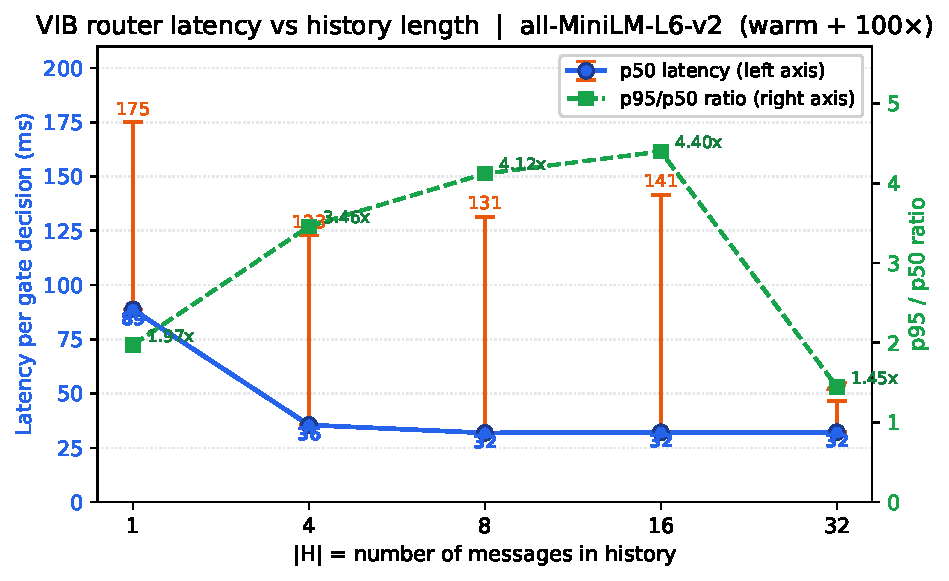
\includegraphics[width=0.72\linewidth]{figures/router_latency.pdf}
\caption{既有离线路由延迟图。Apple M2 Pro、100次预热，历史长度为1、4、8、16、32。分位数比值的变化没有得到因果解释，不能据此给出最优并发或生产延迟承诺。\label{fig:routerlatency}}
\end{figure}

\section{实验协议与主结果}
\subsection{模型、评分与统计}
主实验使用滚动别名\texttt{deepseek-chat}，旧产物无法恢复不可变服务快照。调用层代码对Agent显式设置温度0.2、上限256，对代码合成设置0.1/1024，对数学合成设置0.1/256。因这些参数覆盖客户端默认值，\texttt{t0}文件名不证明真实温度零。

HumanEval执行\texttt{check(candidate)}；MBPP使用顶层断言，不传HumanEval的entry point。旧合成刷新仅定义测试函数而未调用，曾产生100/100假象；独立重评后，主实验HumanEval为151/164与148/164。该错误不能解释所有历史正收益。

MATH用独立\texttt{whole\_answer\_v1}匹配器重评：优先提取最后一个平衡boxed答案，再提取显式答案标签或整条输出；不回退最后数字。保留有序列表、元组、区间开闭，显式集合与union无序比较。常见分数、根式和代数表达式由受限AST与SymPy 1.14.0处理；未知格式保守整文本比较或失败。这不是完整数学语义oracle。

单比例区间使用Wilson方法，差值使用10000次任务配对bootstrap，种子20260812。没有预注册非劣效界值，区间跨零不意味着无损或等效。重复合成先按任务聚合，不把模型调用数当独立任务数。

\begin{table*}[t]
\centering
\caption{三种方法的历史表现与通信预算。VIB相对Full的差值以百分点及配对bootstrap 95\%区间表示；相对Vanilla仅报告点估计。$\dagger$表示区间不跨零；$*$表示主批次McNemar检验$p<0.05$，未经多重检验校正。MBPP因参考测试辅助早停而排除。MATH为保守完整答案匹配率。\label{tab:main_results}}
\setlength{\tabcolsep}{3.4pt}
\scriptsize
\resizebox{\linewidth}{!}{%
\begin{tabular}{@{} l r r r r r r r r r @{}}
\toprule
\textbf{数据集} & \textbf{题数} &
\textbf{Vanilla} & \textbf{Full} & \textbf{VIB} &
\textbf{$\Delta_{\text{V-V}}$} &
\multicolumn{2}{c}{\textbf{$\Delta_{\text{V-F}}$}} &
\textbf{广播} & \textbf{历史Token} \\
& & & & & & \multicolumn{1}{c}{pp} & \multicolumn{1}{c}{95\% CI} & & \\
\cmidrule(lr){7-8}
& & \multicolumn{3}{c}{Pass@1 (\%)} & (pp) & & & \multicolumn{1}{c}{$\downarrow$\%} & \multicolumn{1}{c}{$\downarrow$\%} \\
\midrule

HumanEval       &   164 &   93.90 & 92.07~[+86.91,\,+95.31] & 90.24~[+84.74,\,+93.90] &  -3.66 & -1.83       & [-6.71,\,+3.05] & +21.14 &  +3.88 \\
GSM8K           &  1319 &   59.29 & 95.30~[+94.02,\,+96.32] & 95.22~[+93.93,\,+96.25] & +35.93 & -0.08       & [-0.83,\,+0.68] & +30.49 &  +4.96 \\
MATH            &  5000 &   46.16 & 78.58~[+77.42,\,+79.70] & 77.66~[+76.48,\,+78.79] & +31.50 & -0.92$^\dagger$$^*$ & [-1.78,\,-0.04] & +25.59 &  +4.42 \\
\bottomrule
\end{tabular}}
\vspace{0.3em}
\parbox{\dimexpr\linewidth-2\fboxsep-2\fboxrule\relax}{\sloppy\footnotesize
\textbf{口径说明。}单比例区间使用Wilson方法，差值区间使用10000次任务配对bootstrap。Vanilla的推理预算不与团队对齐；区间跨零不证明等效或非劣效。历史计数减少不等于最终运行的完整费用：HumanEval刷新代码继承旧Token字段，其3.88\%不能作为刷新后完整节省。文件名中的\texttt{t0}不验证真实温度零，不能据此声称温度稳健性。MATH未知格式仍可能漏判。}
\end{table*}


\subsection{主结果解读}
HumanEval的VIB相对Full少3题，差值$-1.83$个百分点，95\%区间$[-6.71,+3.05]$，McNemar $p=0.607$；GSM8K差值$-0.08$个百分点，区间$[-0.83,+0.68]$。这些是未解决的差异，不是已通过非劣效检验。

MATH匹配率为78.58/77.66\%，差值$-0.92$个百分点，区间$[-1.78,-0.04]$，$p=0.04534$。另一记录批次为78.46/77.42\%，差值$-1.04$，区间$[-1.94,-0.10]$，$p=0.03319$。二者未经多重检验校正，且不能解释为采样与真正贪心的对照。

仅由参考答案定义的4458题表达式子集上，两个批次差值为$-0.87$和$-0.90$个百分点，区间分别为$[-1.82,+0.04]$、$[-1.88,+0.09]$，$p=0.06770$、0.07982。负点估计保留，但显著性对覆盖口径敏感；这个事后子集不是新独立验证。

相对历史Vanilla，Full在GSM8K和MATH分别高36.01与32.42个百分点，VIB分别高35.93与31.50个百分点；HumanEval则没有同样优势。因为团队使用更多推理预算，这些差值不能隔离多智能体结构本身的收益。

\begin{figure}[ht]
\centering
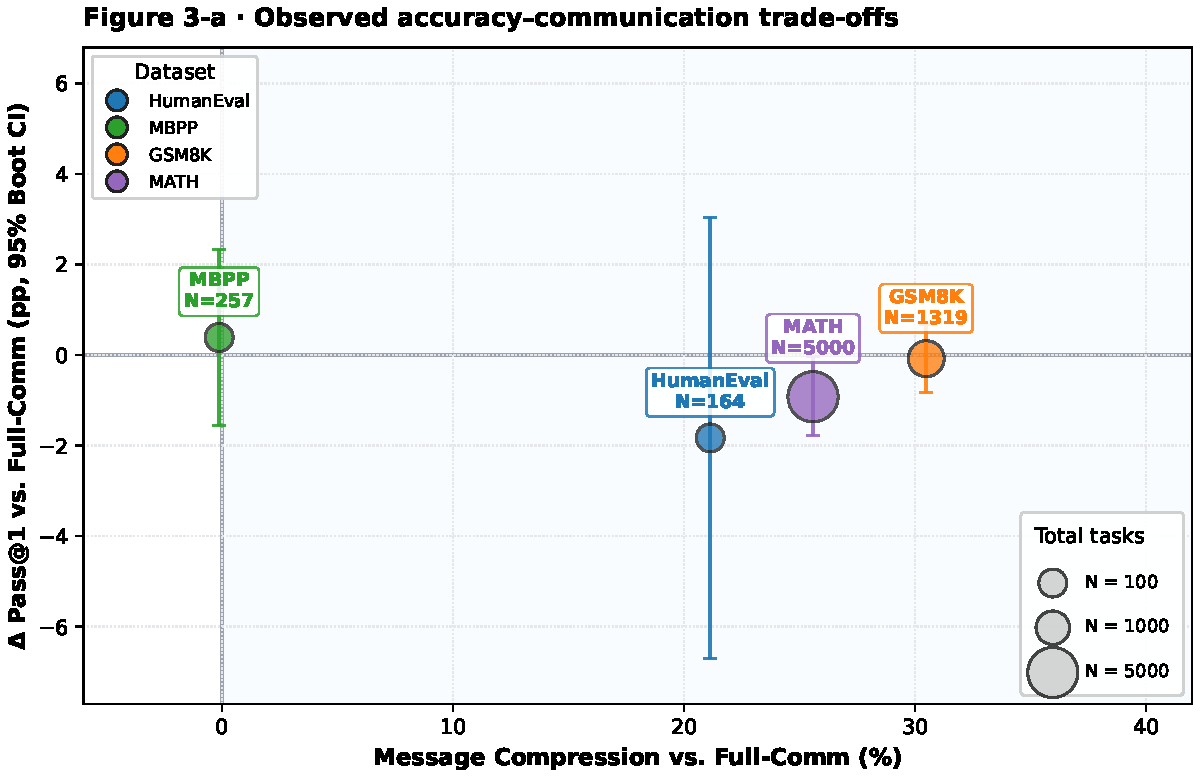
\includegraphics[width=0.76\linewidth]{figures/figure3_pareto_bubble.pdf}
\caption{三个非oracle主基准的广播减少与VIB--Full表现差。误差线为任务配对区间；不同数据集的点不构成同一任务分布下的Pareto前沿，MATH仅表示保守答案匹配结果。\label{fig:pareto}}
\end{figure}

\subsection{角色、简单门控与跨模型证据}
200题GSM8K角色消融中，关闭角色权重的广播减少30.25\%，差值$-0.50$个百分点，区间$[-1.50,0.00]$；开启角色权重时减少25.17\%，差值0.00。不同随机运行及Full精度变动使其不能证明选择性的角色收益。

接近VIB消息预算的余弦阈值0.75减少29.50\%广播，VIB减少30.17\%，两者97.00\%，配对差值区间$[-2.50,+2.50]$。Random减少31.50\%，精度96.00\%，相对VIB差$-1.00$，区间$[-4.00,+1.50]$。余弦门控在实现中名为topk，但实际上是阈值拒绝，不是固定保留$k$条。

Random、VIB和该余弦门控的记录Token减少为13.08\%、5.08\%、4.72\%，表明消息预算接近仍不等于费用相等。三个方法不能据此作等费用优越性判断。

200题网关跨族比较中，DeepSeek参考行和Qwen行差值为$+0.5$和$+1.5$个百分点，消息减少均超过25\%。Qwen为97.50/99.00\%，区间$[0.00,+3.50]$，$p=0.25$。这些是有限迁移观察，不是模型无关保证；网关ID也不独立证明不可变提供方快照。

\section{历史回溯：正收益与实现缺陷}
\subsection{真实正收益并未被重评抹掉}
三个旧HumanEval批次重新执行原entry-point测试后，标签完全保持不变：
\begin{itemize}
\item CLI修正版：Full/VIB为152/155题，即92.68/94.51\%；差值$+1.83$，区间$[-1.83,+5.49]$，$p=0.507812$。
\item 仲裁规则版：148/154题，即90.24/93.90\%；差值$+3.66$，区间$[0.00,+7.32]$，$p=0.109375$。
\item 最少角色救援版：144/149题，即87.80/90.85\%；差值$+3.05$，区间$[-1.83,+7.32]$，$p=0.301758$。
\end{itemize}
加上刷新前主实验，共1312次存档代码检查无标签翻转。这些批次使用已反复调试的同一164题，不能合并制造独立样本，也不能选择最好一次替代当前主表。最高VIB比历史Vanilla仅多1题。

\subsection{刷新改变合成，不是此次门控}
刷新前Full/VIB均147题正确，刷新后为151/148；164题测试与接口逐一一致，两臂328份history、token记录完全一致。Full有45份、VIB有49份最终代码变化。VIB绝对精度从89.63升至90.24\%，只因Full获益更多，相对差值变负。

上述旧正收益批次与刷新前主实验的候选历史各自均不同，因此跨批次94.51到90.24\%的变化不能全归因于一个路由提交。固定输入的旧/当前路由数值探针未发现晚期主配置回归，但使用的是固定测试嵌入，不是实际encoder重放或端到端精度实验。

\subsection{已确认的参数与账目缺陷}
零API RecordingClient配置温度0、上限77后，实际接收到Agent的0.2/256、代码合成0.1/1024、数学合成0.1/256。客户默认值被显式调用参数覆盖，因而必须撤回“真实温度零稳健性”表述。该发现不改变已有输出得分，也不自动解释历史正收益。

合成刷新仅改output和passed，通过旧variant复制保留token字段；94份变化输出继承旧账目。HumanEval的3.88\%只能称历史计数差，不能称刷新后完整费用节省。缺失usage不得通过字符估算偷偷补齐；保持旧字段不变是保存历史，不是证明账单正确。

\subsection{保护配置体现取舍}
在相同5000题、相同完整答案匹配下，数学角色和推理保护都开启的旧批次为78.46/78.32\%，差值$-0.14$，区间$[-1.04,+0.72]$，$p=0.791112$；消息减少5.06\%，记录Token减少0.48\%。主配置关闭保护时为78.46/77.42\%，消息减少25.39\%、Token减少4.21\%。旧评分的$+0.34$在重评后不再保留，但配置存在接近Full精度与更大压缩的取舍。两批不是固定共同候选实验，不能把差值全当保护机制因果收益。

\section{冻结候选重放与公开证据}
\subsection{接收端重放}
两个各24题的历史子集采用任务ID哈希选取，不按pass标签筛题，保留完整两轮六候选。Full、Random、Cosine、VIB、仅首轮、无历史六策略各重复两次，每个数据集288次有效合成，固定网关ID为\texttt{deepseek-v4-flash-0817}。不使用隐藏材料生成答案；HumanEval直接执行entry-point测试，MATH使用严格整答案数值口径。重复先任务内平均，两个数据集不混合。

HumanEval六策略为83.33、87.50、87.50、85.42、91.67、91.67\%。Full相对首轮差$-8.33$，区间$[-20.83,0.00]$；VIB相对首轮$-6.25$，区间$[-20.83,+4.17]$。完整历史可能引入错误，但区间、已见任务和少量差异不支持普遍协作负收益。

MATH所有接收历史的策略为87.50\%，无历史为39.58\%。首轮相对无历史改善14题、恶化1题、持平9题；增加第二轮在任务平均层面没有改善或恶化。首轮的合成Token节省37.35\%，VIB为20.99\%。代理费用为MATH \$0.0389394、HumanEval \$0.1668918，不含历史候选生成，不能当端到端等费用实验。

另取每类24题排除pilot ID，但仍来自已见主基准。Full/首轮/独立同提示控制/无历史各重复两次，每类192次。HumanEval为91.67/95.83/93.75/95.83\%，MATH为95.83/91.67/89.58/75.00\%。Full--首轮为$-4.17$与$+4.17$，区间$[-12.50,0.00]$与$[0.00,+12.50]$，各由1题驱动。同提示控制每类各有1/48评分不同。费用为\$0.105123与\$0.022278。这同时暴露了额外讨论的正负边界及残余随机性，不是已验证的停止策略。

\subsection{公开反例与规格歧义}
HumanEval/93的Full输出违反公开编码例子，错误建议首轮已经存在；不能只归因第二轮。HumanEval/147的Full对公开$n=5$返回4而非1，首轮输出满足该例子。HumanEval/116的32位mask误排非负大整数，但公开例子本身与文字规格冲突，不能声称负数语义已解决。MATH/1791公开面积推导给出最小值16及见证$(1,3,9,3)$，首轮已有正确但不完整推导。

这些证书是事后发现集，不是预测器。全任务字面例子抽取覆盖旧HumanEval 15/24题、新子集8/24题；多解问题要求输出逐字等于示例会误报。规格冲突拒判与多项式残差适配将旧覆盖降为14/24，共同168份输出上Random误报由1/26降至0/26，但Full对基准失败的检出由3/4降至2/4。公开性质通过也可能漏检完整测试失败。

\subsection{输入族、逆变换与接口}
公开多项式契约产生四族各32个有效输入，共128个，开发和验证族各64个。在同一任务12份输出的1536检查中，9份通过全部开发探针，只有1份通过全部验证探针。$x+17$暴露固定搜索区间，$x^3-729$暴露从零起始的Newton导数为零；两个原基准通过输出在新增合法探针失败，属于有限测试覆盖，不是旧check未调用的伪影。输入族不是独立任务。

统一逆变换适配器在两个已见任务16份输出上完成64次往返，共1024检查全部通过；无语义失败分母，不能估计检出灵敏度。其中HumanEval/38缺公开编码helper但解码性质正确，说明接口与算法性质应分开。

接口审计覆盖两批各24题共480输出，288份旧输出全部兼容，新输出191/192兼容，唯一缺失是上述helper。仍有120份旧、112份新输出没有自动语义覆盖。所有输出的讨论决策均标为未评估；接口兼容、有限语义检查、继续讨论选择不是同一个指标。

\section{讨论与研究路线}
现有证据支持：生成后门控可减少广播；VIB保留较多团队效果；历史正收益是真实观察；复杂门控尚未稳定超越简单规则。它既不证明VIB工作无价值，也不证明恢复最好历史版本就能获得可靠方法优势。

局限包括滚动模型别名、短小三角色团队、已见任务调参、非等费用Vanilla、事后选择、MATH语义匹配覆盖不足、温度参数透传、刷新费用缺失、oracle早停及多重检验。区间跨零不能视作无损，显著负差也不能不顾评分覆盖与配置差异作普遍结论。

下一阶段顺序为：
\begin{enumerate}
\item 修复stage参数贯通和输出--usage关联，先用零API RecordingClient、幂等账目与失败恢复测试验证，不改历史结果。
\item 固定已有候选流，对旧简洁提示、现有仲裁提示和公开规格优先提示进行单因素重复合成。Reviewer错误被放大是待验证假设，隐藏测试只作事后评分。
\item 通过题面/参考哈希去重，冻结研究者未用于设计的新任务。研究者未见不等于模型未训练过。
\item 引入预算受限单智能体self-refine、Full、首轮和简单门控，比较相同实际费用下的任务表现，而非仅费用上限或消息数相同。
\end{enumerate}
建议先校准后报价，探索初始整体费用上限\$3；这不是保证完成大样本验证的报价。80题不能保证检测1个百分点，更不足以无条件证明非劣效，确认实验须提前做功效分析。本文没有运行这批新付费实验。

\section{相关工作}
AgentCoder、ChatDev、MetaGPT、SWE-agent和OpenDevin涉及代理软件工作流\citep{du2023agentcoder,qian2023chatdev,hong2023metagpt,yang2024sweagent,wang2024opendevin}。DyLAN、LLMLingua、AgentPrune与AgentDropout涉及团队优化、提示压缩或通信裁剪\citep{liu2023dylan,jiang2023llmlingua,zhang2024agentprune,wang2025agentdropout}，因此稀疏通信本身不能声称新颖。本文没有在相同harness下复现这些方法的主结果。

信息瓶颈、深度VIB和InfoBERT关注信息保留及正则化\citep{tishby2015deep,alemi2017variational,wang2021infobert}，与本文启发式的理论强度不同。Self-Refine提示应设置强单智能体迭代对照\citep{madaan2023selfrefine}；关于多智能体辩论评估的研究也强调推理预算和模型差异\citep{zhang2025stopovervaluing}。StreamingLLM及MemWalker主要研究长上下文或记忆导航\citep{xiao2023streamingllm,liu2024memwalker}，不等同于本文短团队广播门控。

\section{结论}
本文不是宣称VIB稳定优于Full或简单门控，而是展示可观测的通信权衡与影响结论的协议边界。历史正收益应保留、复现和解释，负差值也应如实披露。先修可复现性和费用关联，再开展固定候选提示词实验及独立等实际费用验证，是保留已有研究价值、避免盲目扩样的更可靠路径。

\clearpage
\appendix
\section{历史MBPP：oracle-only结果}\label{app:gate_trace}
257题Full/VIB为91.83/92.22\%，$p=1.0$，消息与Token分别增加0.12\%、0.05\%。OR分组为236题Early-Stopped、21题Multi-Round，取决于两臂实际结果。前组99.15/98.73\%，后组9.52/19.05\%，不构成预先确定困难任务上的确认收益。前组消息变化实际为$-0.41\%$，不能硬编码零。参考测试参与早停、废弃probe费用可能遗漏，故不进入主结果。

MBPP/260与285的VIB通过、Full失败，但两臂均广播6/6，历史没有逐候选分数日志。这说明随机产物不同，不能说明VIB过滤了错误测试，也不能用后版路由重建缺失证据。

\section{复现声明}\label{app:repro}
主表数值由\path{scripts/export_latex_tables.py}读取修正JSON生成，中英文共用每行数值；图共用既有资产。MATH主实验、Vanilla、重跑均保留原文件、source/script/matcher哈希、逐题新旧标签和非标签字段不变性摘要。主实验Full 177条false变true、252条true变false，VIB为181与256；这些是匹配判定变化，不全是人工确认的纠错。

参考-only分类为4458表达式、253 opaque、289结构化答案。主批9条、Vanilla 14臂记录（7份不同输出）、重跑6条有提取或格式异常。单位、百分数、自然语言、等价方程和未显式标为集合的无序答案仍可能漏判。在线旧MATH/GSM8K评分分派未在本轮修改，新实验须冻结协议，不能把旧标签续跑到新协议。

门控分数在相同输入下确定，不控制外部模型随机性。Full四个200题批次94.5、95.5、96.5、97.0\%是2.5个百分点观察范围，不是置信区间。缓存、请求身份和输入协议应幂等；协议漂移、缺usage、截断或网关失败不应静默计成合法结果。

\paragraph{后续工程修复。}
零API测试现已截获Agent、团队与Vanilla合成及代码修复重试的实际请求，确认显式全局和分阶段参数能够透传；省略参数仍保留历史stage默认。新增追加式请求账目关联参数、prompt和输出哈希、响应标识及已知usage；缺usage和未完成请求仍标未知。新运行保留废弃probe账目，新刷新关联parent输出与新增请求，不声称补回历史完整费用。这是面向未来运行的工程验证，没有新增模型性能或货币节省证据。

\paragraph{预算与恢复组件。}
独立SQLite会话冻结请求spec、评测版本和代理价目；零API测试覆盖多worker及独立数据库连接的原子预留、未知请求停机和已收到响应的缓存复用。预算保证以经验证的prompt Token上界及提供方输出上限为条件；超界时保留实际用量并停机。已收到输出可只恢复本地评测，缺usage则保留预留。此组件并不意味着旧benchmark driver已经完成端到端迁移；代理价格校准、完整driver接入及因果对照清单仍须付费验证前验收。

\section{伦理、作者与投稿元数据}\label{app:ethics}
研究使用公开代码与数学基准，没有受试者实验。作者署名为屈占祥，独立研究者，联系邮箱为\texttt{zhanxiangqu@126.com}；性别和年龄不进入学术署名或实验数据。

门控不是安全机制，错误近义建议可通过，关键修正可被丢弃；代码生成具有基础模型相关的双重用途风险。本文没有测量能耗、碳排或生产P99，不把Token计数自动等同这些收益。公开数据权限、准确许可证及目标期刊模板仍须投稿前复核。

\paragraph{资助声明。}本研究未获得外部资助。
\paragraph{利益冲突声明。}作者声明不存在利益冲突。
\paragraph{研究者标识。}作者提供的ORCID为\href{https://orcid.org/0009-0000-0137-9751}{0009-0000-0137-9751}，姓名为Zhanxiang Qu。格式与校验位已离线核对，但未独立核验线上身份资料。该标识用于区分同名研究者和关联研究成果，不代表学术资格认证。

\section{文档导航}
\begin{tabular}{@{}lp{0.68\linewidth}@{}}
\toprule
入口 & 用途 \\
\midrule
\href{paper.pdf}{英文论文} & 英文研究工作稿；正式投稿仍需官方模板和独立验证。\\
\href{paper_zh.pdf}{中文论文} & 本文；中文叙述与英文事实口径对应。\\
\href{gap1_claim_audit_trail.md}{研究审计与路线} & 历史提交、重评结果、参数与成本问题、下一阶段预算门。\\
\href{../scripts/export_latex_tables.py}{生成表格} & 中英文主表共同事实源，禁止手改生成的表格。\\
\bottomrule
\end{tabular}

\bibliographystyle{apalike}
\bibliography{refs}
\end{document}
